\chapter{Theorie}
\label{ch:theory}
Zu Beginn der Arbeit werden zunächst die zwei Modelle zur Beschreibung der Herzdynamik eingeführt, auf die die verschiedenen Ansätze angewendet werden. Im Anschluss daran werden zunächst die theoretischen Grundlagen der klassischen Methoden der \textit{nächsten Nachbar} Vorhersage und der \textit{radialen Basisfunktionen} zusammengefasst. Darauffolgenden wird der Ansatz des \textit{Reservoir Computings} eingeführt und theoretisch anhand der \textit{Echo State Networks} beschrieben.

\section{Modelle des Herzens}
Zur Beschreibung der Herzdynamik existieren verschiedene Modelle. In dieser Arbeit werden zuerst das \textit{Barkley}- und das \textit{Mitchell-Schaeffer}-Modell verwendet, um die Leistungsfähigkeit der \textsc{ESN}s zu überprüfen und einzuordnen. Anschließend werden die gewonnenen Erkenntnisse auf das kompliziertere \textit{Bueno-Orovio-Cherry-Fenton}-Modell angewendet. Im Folgenden sollen die drei Modelle vorgestellt werden.

\subsection{Barkley-Modell}
Das \textit{Barkley}-Modell, welches 1990 von Dwight Barkley vorgestellt wurde, ist ein System aus gekoppelten Reaktionsdiffusionsgleichungen. Dies sind partielle Differentialgleichungen (\textit{PDE}) zweiter Ordnung, welche einen Diffusionsterm besitzen. Das \textit{Barkley}-Modell beschreibt ein erregbares und oszillierendes Medium. Das Modell besteht aus zwei Variablen $u(t)$, $v(t)$ die den  \textit{PDEs}
\begin{equation}
\begin{gathered}
\frac{\partial u}{\partial t} = D \cdot \nabla^2 u + \frac{1}{\epsilon} (1-u) \left(u-\frac{v+b}{a}\right)\\
\frac{\partial v}{\partial t} = u^\alpha-v,
\end{gathered}
\end{equation}
unterliegen \citep{Barkley:2008}. Dabei ermöglicht $\alpha=1$ dem System \textit{periodische} Wellenmuster auszubilden und $\alpha=3$ bedingt ein \textit{chaotisches} Verhalten. Im Folgenden wird stets der Fall $\alpha=3$ betrachtet. Die Variable $u(t)$ durchläuft hierbei eine schnellere Dynamik als die hemmende Variable $v(t)$ \citep{Barkley:2008, berg2011synchronization}. Das Modell kann genutzt werden, um die Dynamik der Herzgewebes zu beschreiben. Dabei nimmt die Variable $u$ die Rolle einer Membranspannung ein.\\
Die Parameter $\epsilon, b$ und $a$ charakterisieren das Verhalten des Systems und werden in der gesamten folgenden Arbeit nach \citep{Barkley:2008} als
\begin{align*}
a &= 0.8,\\ b &= 0.01,\\ \epsilon &= 0.02
\end{align*}
festgelegt.\\
Zudem wird das Modell in dieser Arbeit in zwei Dimensionen betrachtet, sodass $u(t, x,y)$ und $v(t, x,y)$ skalare zeitabhängige Felder sind.\\
Die \textit{PDE}s werden zunächst zur Simulation des Systems zeitlich mit einem Zeitschritt $\Delta t$ und örtlich mit einer Gitterkonstante $\Delta x$ diskretisiert. Zur Beschreibung des Diffusionstermes wird eine Fünf-Punkte Methode
\begin{align}
\nabla^2 u(t)_{i,j} \simeq \frac{u(t)_{i-1, j} + u(t)_{i+1,j} + u(t)_{i,j-1} + u(t)_{i,j+1} - 4 u(t)_{i,j}}{\Delta x^2} \eqdef \Sigma(t)_{i,j}
\end{align} 
nach \citep{Barkley:2008} verwendet. Die tiefergestellten Indizes stehen für den diskretisierten Ort der \textit{x-y-Ebene}.
Für kleine Zeitschritte $\Delta t$ ist ein \textit{explizites Eulerverfahren}
\begin{equation}
\begin{gathered}
u(t+1)_{i,j} = u(t)_{i,j} + \Delta t \cdot \frac{\partial u}{\partial t},\\
v(t+1)_{i,j} = v(t)_{i,j} + \Delta t \cdot \frac{\partial v}{\partial t}
\end{gathered}
\end{equation}
mit

\begin{equation}
\begin{gathered}
\frac{\partial u}{\partial t}_{i,j} = D \cdot \Sigma(t)_{i,j} + \frac{1}{\epsilon} (1-u(t)_{i,j}) \left(u(t)_{i,j}-\frac{v(t)_{i,j}+b}{a}\right)\\
\frac{\partial v}{\partial t}_{i,j} = u(t)_{i,j}^3-v(t)_{i,j}
\end{gathered}
\end{equation}
ausreichend genau. Hierbei werden \textit{Neumann}-Randbedingungen genutzt, sodass die senkrechte Komponente der räumlichen Ableitung an den Rändern des Feldes verschwindet. Im Folgenden wird zudem, in Analogie zu \citep{berg2011synchronization}, die Diffusionskonstante auf $D = 1/25$, die Gitterkonstante auf $\Delta x = 0.1$ und die Zeitkonstante auf $\Delta t = 0.01$ gesetzt. Die raumzeitliche Dynamik des Systems ist in Form der $u$-Variable im Anhang in Abbildung \ref{fig:apx_barkley_evolution} dargestellt.
\section{Mitchell-Schaeffer Modell}
Das \textit{Mitchell-Schaeffer Modell} ist ebenso wie das \textit{Barkley Modell} ein System aus gekoppelten partiellen Differentialgleichungen. Es ist vorgeschlagen worden, um eine phänomenologisches Beschreibung der Aktionspotentiale auf der Membran von Herzzellen zu liefern. Das Modell wird durch die Membranspannung $v(t)$ und eine Kontrollvariable $h(t)$, welche das Verhalten der beteiligten Ionenkanäle steuert, definiert. Hierbei wird die Spannung als dimensionslose Größe dargestellt, die Werte zwischen $0$ und $1$ annehmen kann \citep{mitchell2003two}.\\

Diese Dynamik wird durch die Gleichungen 
\begin{equation}
\begin{gathered}
\frac{\partial v}{\partial t} = \nabla \cdot (D \nabla v) + \frac{h v^2(1-v)}{\tau_{in}} - \frac{v}{\tau_{out}},\\
\frac{\partial h}{\partial t} =
\begin{cases}
	\frac{1-h}{\tau_{open}},& \text{wenn } v \leq v_{gate}\\
    \frac{-h}{\tau_{close}},& \text{wenn } v \geq v_{gate}
\end{cases}
\end{gathered}
\end{equation}
beschrieben. Dabei stehen die Parameter $\tau_{in}, \tau_{out}, \tau_{open}, \tau_{close}$ für Zeitkonstanten, welche die Form des Aktionspotentials modifizieren. Die ersten beiden Konstanten beschreiben die Geschwindigkeit, mit der die Ionen durch die Membran strömen, und die letzten beiden die Geschwindigkeit mit der sich die verantwortlichen Ionenkanäle öffnen beziehungsweise schließen. Zusätzlich stellt die Konstante $v_{gate}$ eine Grenzspannung dar. Beim Über- und Unterschreiten dieser Grenze ändert sich der der jeweilige Zustand der Ionenkanäle , indem $h(t)$ angepasst wird. Im Rahmen dieser Arbeit werden, soweit keine anderen Angaben vorhanden sind, die Parameter durch die Werte aus Tabelle \ref{tab:ms_parameters} in Analogie zu \citep{mitchell2003two} festgesetzt. Dabei ist allerdings $\tau_{open}$ auf $20$ \citep[S. 134ff.]{bartocci2016computational} reduziert worden, da mit dieser Wahl ein chaotischeres Verhalten, ähnlich zum \textit{Barkley-Modell}, erzeugt wird. Dies erschwert die mögliche Vorhersage der Entwicklung, wodurch eine anspruchsvolle Herausforderung erzeugt wird.\\

\begin{table}[H]
\centering
\begin{tabular}{|c|c|c|c|c|}
$\tau_{in}$ & $\tau_{out}$ & $\tau_{open}$ & $\tau_{close}$ & $v_{gate}$ \\ 
\hline 
\hline 
0.3 & 6.0 & 20 & 150 & 0.13 \\ 
\hline 
\end{tabular} 
\caption{Verwendete Zeitkonstaten und Grenzspannung $v_{gate}$ für die Betrachtung des \textit{Mitchell-Schaeffer Modells}}
\label{tab:ms_parameters}
\end{table}

Der erste Summand der zeitlichen Ableitung von $v$ beschreibt ein Diffusionsverhalten, welches durch die Diffusionsmatrix $\mathbf{D} = \text{diag}(D_x, D_y)$ beschrieben wird. Die Einführung dieser Matrix erlaubt im Allgemeinen die Verwendung von zwei verschiedenen Diffusionskontanten $D_x, D_y$, welche Richtungsabhängig sind \citep{talbot2013towards}. Im Folgenden wird für diese allerdings der gleichen Wert $D_x = D_y = D$ gesetzt.\\

Die meisten, auf zellulärer Ebene aufgestellten, Gleichungen haben eine hohe Komplexität. Hierdurch werden numerische Berechnungen sehr aufwendig. In der Herleitung dieses Modells sind einige vereinfachende Annahmen eingeflossen, wodurch die Komplexität und somit auch der numerische Aufwand reduziert worden sind. Trotz des phänomenologischen Charakters des \textit{Mitchell-Schaeffer Modells} besitzen die Parameter eine physiologische Interpretation. Zudem ist es in der Lage wichtige Eigenschaften des Aktionspotentials im Vergleich zu anderen Modellen gut wiederzugeben \citep{talbot2013towards}.\\

Analog zu der Betrachtung des \textit{Barkley Modells} sind für die numerische Betrachtung die beiden \textit{PDE}s erneut in einem expliziten Verfahren mittels
\begin{equation}
\begin{gathered}
\frac{\partial v}{\partial t}_{i,j} = D \cdot \Sigma(t)_{i,j} + \frac{h(t)_{i,j} v(t)_{i,j}^2(1-v(t)_{i,j})}{\tau_{in}} - \frac{v(t)_{i,j}}{\tau_{out}}\\
\frac{\partial h}{\partial t}_{i,j} = \begin{cases}
	\frac{1-h(t)_{i,j}}{\tau_{open}},& \text{wenn } v(t)_{i,j} \leq v_{gate}\\
    \frac{-h(t)_{i,j}}{\tau_{close}},& \text{wenn } v(t)_{i,j} \geq v_{gate}
\end{cases}
\end{gathered}
\end{equation}
diskretisiert worden. Dabei werden im Folgenden die Integrationskonstanten $\Delta x = 0.1, \Delta t = 0.01$ und die Diffusionskonstante $D_x = D_y = D = \num{5e-3}$ genutzt.\\
\subsection{Bueno-Orovio-Cherry-Fenton-Modell}
Ebenso wie die beiden vorherigen Modelle ist das \textit{Bueno-Orovio-Cherry-Fenton}-Modell (\textit{BOCF}-Modell) ein System aus gekoppelten partiellen Differentialgleichungen. Es ist ein sogenanntes \textit{minimales Modell} zur Beschreibung der Aktionspotentiale auf der Membran von Herzzellen. Dies bedeutet, dass nicht jeder einzelne Ionenstrom modelliert wird, sondern diese in drei verschiedene Gruppen unterteilt und diese dann zusammen modelliert werden: Dabei werden sie in \textit{schnell hineinströmende}, \textit{langsam hineinströmende} und \textit{ausströmende} Ionen unterteilt. Dieses Vorgehen reduziert die Anzahl der benötigten Variablen des Systems sehr stark: Während andere Modelle auf Ionenebene zur Beschreibung der Aktionspotentiale viele Variablen besitzen, wie beispielsweise das \textit{Tuscher-Noble-Noble-Panfilov}-Modell (\textit{TNNP}-Modell) mit $17$ Variablen, benötigt das \textit{BOCF}-Modell nur $4$ Variablen - dies senkt den benötigten Rechenaufwand. Gleichzeitig beinhaltet es $28$ Konstanten, welche die Form der Dynamik charakterisieren. Dadurch ist zum einen eine Anpassung an verschiedene experimentelle Messergebnisse möglich, zum anderen können auch die Ergebnisse anderer bestehender Modelle reproduziert werden. Hierdurch kommt die Bezeichung des \textit{minimalen Modells} zustande \citep{Bueno-Orovio2008}.\\

Die Dynamik wird durch die Gleichungen 
\begin{align}
\begin{aligned}
\frac{\partial u}{\partial t} &= D \nabla^2 u - (J_{si} + J_{fi} + J_{so})\\
\frac{\partial v}{\partial t} &= \left(1-H(u-\theta_w)\right)(v_\infty - v)/\tau_v^- - H(u-\theta_v)v/\tau_v^+ \\
\frac{\partial w}{\partial t} &= (1-H(u-\theta_w))(v_\infty - w)/\tau_v^- - H(u-\theta_w)v/\tau_w^+ \\
\frac{\partial s}{\partial t} &= ((1 + \tanh(k_s(u-u_s)))/2 - s)/\tau_s
\end{aligned}
\end{align}
beschrieben. Die drei Ströme $J_{si}$, $J_{fi}$ und $J_{so}$ folgen den Gleichungen
\begin{align}
\begin{aligned}
J_{si} &= -H(u-\theta_w)ws/\tau_{si} \\
J_{fi} &= -vH(u-\theta_v)(u-\theta_v)(u_u - u)/\tau_{fi} \\
J_{so} &= (u-u_o)(1-H(u-\theta_w))/\tau_o + H(u-\theta_w)/\tau_{so}.
\end{aligned}
\end{align}

Dabei steht $H(x)$ für die \textit{Heaviside-Funktion}. Zusätzlich werden sieben spannungsabhängige Konstanten
\begin{align}
\begin{aligned}
\tau_v^-   &= (1-H(u-\theta_v^-))\tau_{v1}^- + H(u-\theta_v^-)\tau_{v2}^- \\
\tau_w^-   &= tau_{w1}^- + (\tau_{w2}^- - \tau_{w1}^-)(1+\tanh(k_w^-(u-t_w^-)))/2 \\
\tau_{so}^- &= tau_{so1}^- + (\tau_{so2}^- - \tau_{so1}^-)(1+\tanh(k_{so}^-(u-t_{so})))/2 \\
\tau_s^-    &= (1-H(u-\theta_w))\tau_{s1} + H(u-\theta_w)\tau_{s2} \\ 
\tau_o^-    &= (1-H(u-\theta_o))\tau_{o1} + H(u-\theta_o)\tau_{o2} \\\\
v_\infty &= \begin{cases}
	1,& \text{wenn } u \leq \theta_v^-\\
    0,& \text{wenn } u \geq \theta_v^-
\end{cases} \\
w_\infty &= (1-H(u-\theta_o))(1-u/\tau_{w\infty}) + H(u-\theta_o)w_\infty^*
\end{aligned}
\end{align}
eingeführt. In diesem Modell beschreibt die Variable $u(t)$ die Membranspannung. Des Weiteren wird das Modell durch $28$ Konstanten charakterisiert. In dieser Arbeit wird der Satz von Konstanten genutzt, welcher das \textit{Tuscher-Noble-Noble-Panfilov}-Modell reproduziert. Die Konstanten sind in \ref{tab:apx_bocf_tnpp_constants} zu finden. Sie sind ausgewählt worden, weil mit ihnen eine chaotische Dynamik beobachteten werden kann \citep{Bueno-Orovio2008}.\\

Die Differentialgleichungen sind erneut, wie zuvor auch im \textit{Barkley}- und im \textit{Mitchell-Schaeffer}-Modell, diskretisiert worden. Zudem werden die gleichen Randbedingungen genutzt. Im Folgenden werden die Integrationskonstanten $\Delta x = 1.0, \Delta t = 0.1$ und die Diffusionskonstante $D = \num{2e-1}$ verwendet. Die raumzeitliche Dynamik des Systems ist in Form der $u$-Variable im Anhang in Abbildung \ref{fig:apx_bocf_evolution} dargestellt.\\


\clearpage
\section{Klassische Methoden}
Als nächstes sollen nun die bisherigen Ansätze auf dem Gebiet der (raum)zeitlichen Vorhersage vorgestellt werden. Hierzu wird zuerst die Technik der \textit{Verzögerungskoordinaten} eingeführt, welche die Grundlage der Methoden der \textit{Nächsten-Nachbar}-Vorhersage und der \textit{radialen Basisfunktionen} bildet.
 
\subsection{Verzögerungskoordinanten}
\label{sc:delay_reconstruction}
Die \textit{Verzögerungskoordinaten} (Delay Coordinates) können benutzt werden um Zeitreihen zu analysieren und den Phasenraum des ursprünglichen Systems zu rekonstruieren.
Hierbei wird ein Signal $s(t)$ an diskreten Zeitpunkten betrachtet, sodass sich das diskrete Signal $s_n = s(n\Delta t)$ ergibt. Eine solche Rekonstruktion erzeugt hieraus ein Signal, in welchem die Informationen $\delta$ vorheriger Zeitpunkte mit dem Abstand $\tau$ enthalten sind. Somit wird eine höherdimensionale Zeitreihe $\vec{z}_n \in \mathbf{R}^{\delta}$ durch
\begin{align}
	\vec{z}_n = \left(s_{n-(\delta-1)\tau}, s_{n-(\delta-2)\tau}, \ldots ,s_n \right)
\end{align} 
konstruiert \citep[35\,ff.]{kantz2004nonlinear}. Bei einer ausreichend hohen Wahl der Rekonstruktionsdimension $m$ ist es hiermit möglich den Phasenraum des Attraktors zu rekonstruieren. Für die Wahl der Verzögerungszeit $\tau$ gibt es keine rigorose mathematische Definition oder Beschreibung, sondern es existieren verschiedene Ansätze zur Ermittlung des optimalen Wertes. Ein populärer Ansatz, welcher in dieser Arbeit verwendet wird, besteht darin, $\tau$ durch das Auffinden der ersten Nullstelle der Autokorrelationsfunktion 
\begin{align}
AUC(\tau) = \sum_l^{N-\tau} (s_l-\bar{s})(s_{l+\tau}-\bar{s})
\end{align}   
zu ermitteln. Dies lässt sich dadurch motivieren, dass durch das Hinzunehmen von Signalen der Zeitreihe, die um diesen Wert $\tau$ verschoben sind, am meisten neue Information hinzugefügt wird, da die Selbstähnlichkeit des Signals am geringsten ist \citep[30\,ff.]{kantz2004nonlinear}.
Die so konstruierte höherdimensionale Zeitreihe beinhaltet somit also nicht nur Informationen über den aktuellen Zustand des Systems, sondern auch über die unmittelbare Vergangenheit. Dadurch können diese rekonstruierten Datenpunkte auch genutzt werden, um das Verhalten dynamischer Systeme vorherzusagen. Hierfür werden im Folgenden zwei Methoden eingeführt.
\subsection{Nächster Nachbar Vorhersage}
\label{sc:theory_nn}
Die erste Methode um mittels der zuvor konstruierten höherdimensionalen Zeitreihen Vorhersagen zu treffen ist die \textit{nächste Nachbar}-Vorhersage (im Folgenden als \textsc{NN}-Ansatz abgekürzt). Das allgemeine Ziel \textit{NN}-Vorhersage besteht darin den funktionalen Zusammenhang $F : X \rightarrow Y$ zu finden, welcher Daten der Menge $X \in \mathbb{R}^n$ auf Elemente aus $Y \in \mathbb{R}^m$ eindeutig abbildet. Hierfür wird angenommen, dass die Funktion $F$ lokal stetig ist. Zudem werden hierfür Daten benötigt, anhand derer der Zusammenhang erlernt werden kann. Die Anzahl dieser Trainingsdaten wird im Folgenden mit $N$ bezeichnet.\\
Zu Beginn werden Paare $(\vec{x},\vec{y}) \in X \times Y$ aus einem \textit{Trainingsdatensatz} gebildet und eine Suchstruktur über die $x$-Werte gebildet. Nun kann diese Struktur genutzt werden, um für ein gegebenes $\vec{x}$ den wahrscheinlichsten Wert $\vec{y}$ zu suchen. Hierfür werden, unter der Annahme der lokalen Stetigkeit, die Datenpunkte $\vec{x}_1, ..., \vec{x}_k$ aus der zuvor angelegten Suchstruktur ausgewählt, welche den geringsten Abstand $d(\vec{x}, \vec{x_i})$ zu $\vec{x}$ besitzen.\\
Diesen $k$ Datenpunkten ist jeweils ein eindeutiger Wert $\vec{y}_i$ zuvor zugeordnet werden. Damit kann nun eine Approximation für den zu $\vec{x}$ gehörigen Wert $\vec{y}$ erstellt werden, indem beispielsweise ein gewichteter Mittelwert der $\vec{y}_i$ genutzt wird. Hierzu kann jedem der $k$ nächsten Nachbarn $(\vec{x}_i, \vec{y}_i)$ ein Gewicht $w_i(\vec{x})$ nach
\begin{align*}
w_i(\vec{x}) = \frac{v_i}{\sum_j v_j}, \text{ mit } v_i = \frac{1}{||\vec{x}_i-\vec{x}||} 
\end{align*}
zugeordnet werden. Diese Definition erfüllt $\sum_i w_i = 1$ und ordnen zudem fernen Nachbarn ein geringeres Gewicht zu. Die dabei auftretende Norm $||\cdot ||$ wird im Folgenden als euklidisch angenommen, sofern keine weiteren Angaben existieren. Somit ergibt sich für die gewichtete Vorhersage
\begin{align}
F(\vec{x}) = \vec{y} = \sum^k_i \vec{y}_i \left( \sum_j \frac{||\vec{x}_i-\vec{x}||}{||\vec{x}_j-\vec{x}||} \right) ^{-1}.
\end{align}

Der Schlüssel in der Bewältigung einer solchen Aufgabe liegt hauptsächlich in der Art und Weise, wie die $k$ nächsten Nachbarn gesucht werden. Hierbei wird im Folgenden ein naiver Ansatz ebenso wie der Algorithmus \textsc{k-d-tree} betrachtet. Bei dem naiven Ansatz (\textit{brute force}) werden die nächsten Nachbarn aus dem unsortierten Trainingsdatensatz durch pures Ausprobieren aller möglichen Punkte ermittelt.

\subsubsection{k-d-tree}
Ein \textsc{k-d-tree} ist eine Spezialform eines Binärbaumes, und eine oftmals genutzte Methode um Suchvorgänge in Datenstrukturen durchzuführen. Das zugrundeliegende Prinzip eines solchen Baumen ist, dass wenn der Punkt $P_1$ weit entfernt von $P_2$ liegt, aber $P_3$ nahe an $P_2$ liegt, so folgt daraus, dass $P_1$ und $P_3$ weit voneinander entfernt liegen müssen. Durch eine solche Argumentation muss bei einem solchem Suchvorgang die Distanz zweier Punkte seltener berechnet werden, wodurch Rechenzeit eingespart werden kann.\\

\begin{figure}[h]
    \centering
    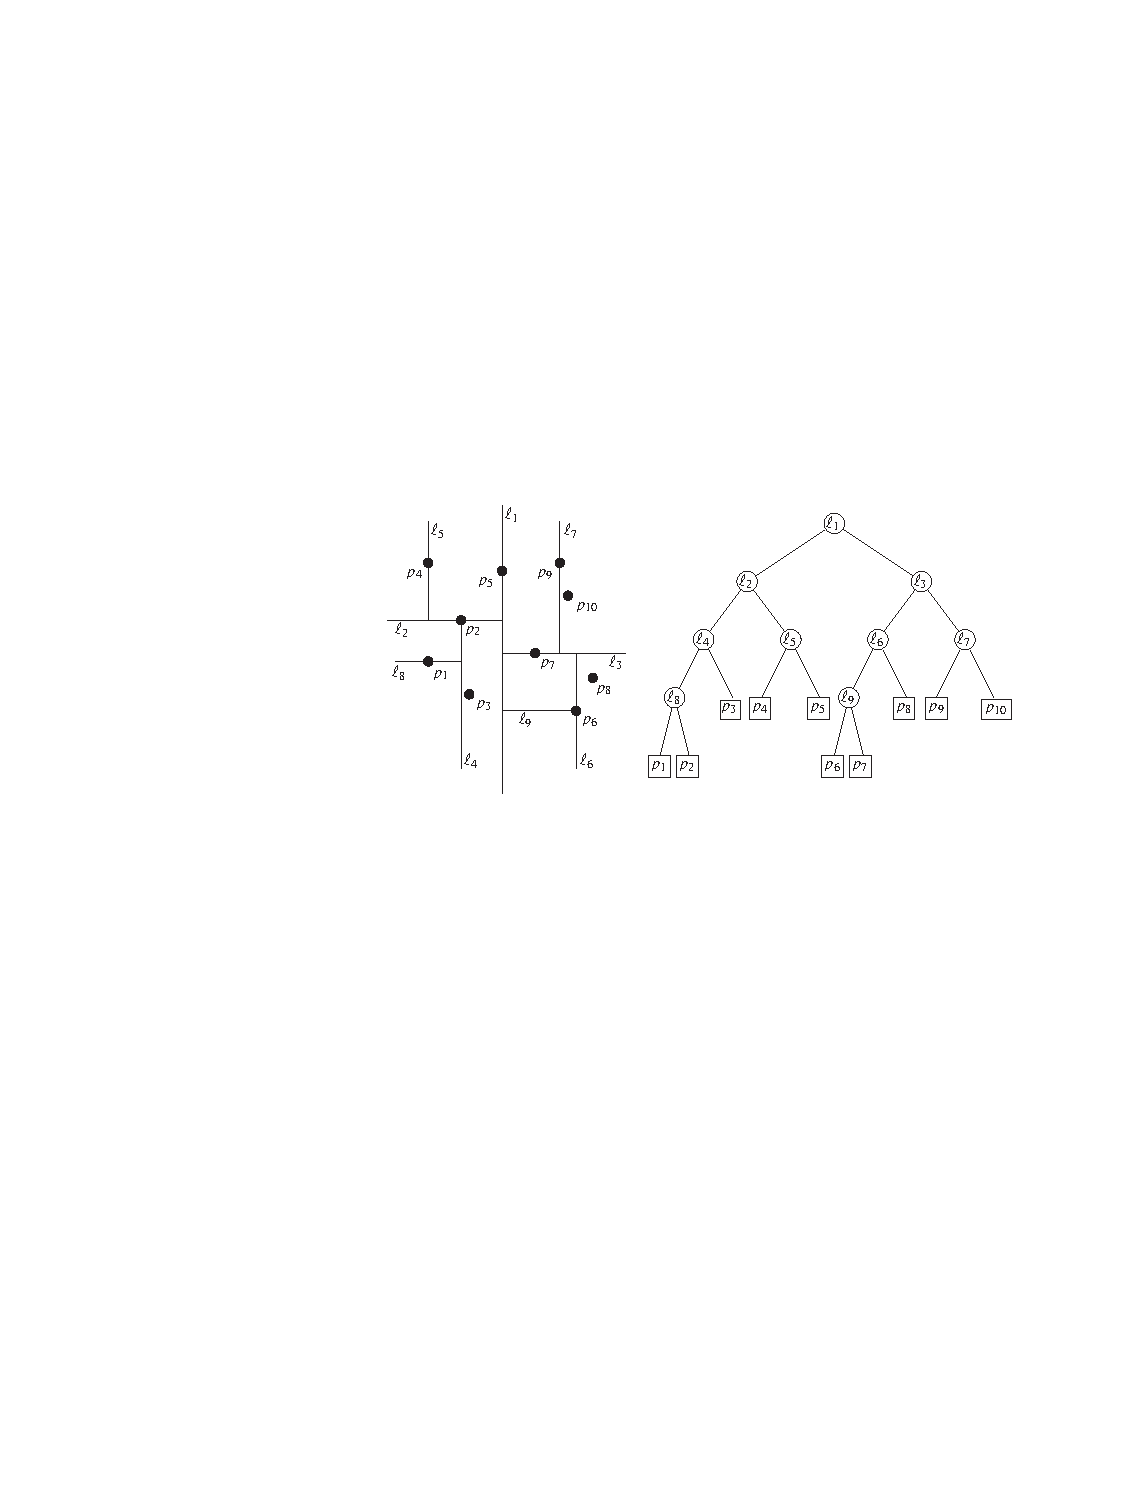
\includegraphics[width = 0.9 \textwidth]{figures/illustrations/kdtree.pdf}
    \caption{Exemplarische Darstellung eines \textsc{k-d-trees} für $d=2$ Dimensionen. In der linkten Hälfte ist die graphische Interpretation der Aufteilung und in der rechten der Aufbau des entstehenden Baumes zu finden \cite{de2000computational}. Der in der $i$-ten Iteration bestimmte Median ist als $l_i$ eingetragen. An jeder Astgabelung werden die Elemente falls sie kleiner als der Median $l_i$ sind in den linken und ansonsten in den rechten Zweig einsortiert.}
    \label{fig:kdtree}
\end{figure}

\improvement{Add search path example to the graph?}

Der Suchvorgang besteht aus zwei Phasen. Zuerst wird die Aufbauphase des Baumes durchgeführt, bei der die Trainingsdaten einsortiert und damit ein Suchindex erzeugt wird. Anschließend folgt die Suchphase, bei der der zuvor erstellte Suchindex nach dem nächsten Nachbarn durchsucht wird.\\

In der Aufbauphase wird zuerst eine Dimensionen ausgewählt und der Median $l_i$ der Daten in dieser Dimension bestimmt. Dieser Wert bildet eine Trennlinie, anhand derer die Punkte in zwei Mengen unterteilt werden, die entweder nur größere oder nur kleinere Elemente bezogen auf jene Dimension beinhalten. Die beiden Mengen bilden die ersten Äste des Baumes. Nun wird dieser Schritt rekursiv auf alle Äste angewendet, und die hierbei zum Vergleich genutzte Dimension iteriert \cite{de2000computational}. Dieses Verfahren wird so lange wiederholt, bis eine bestimmte maximale Anzahl $N_{max}$ an Knotenpunkten pro Ast erreicht wird. Ab dieser unteren Grenze wird das Erstellen des Binärbaumes beendet. Ab dieser Grenze benötigt der Zugriff auf die verschiedenen Elemente und das Aufteilen in neue Äste mehr Zeit, als das Berechnen der Abstände zwischen den verbleibenden $N_{max}$ Knoten und dem Suchpunkt. Eine beispielhafte Darstellung des Verfahrens ist in Abbildung \ref{fig:kdtree} zu finden.

Die Suchphase wird nun wieder rekursiv durchgeführt. Hierbei werden wieder iterierend die verschiedenen Dimensionen verglichen, und sich somit immer weiter im Suchbaum nach unten ein Weg gebahnt \cite{de2000computational}. In der untersten Ebene, also wenn nur noch eine Suche zwischen maximal $N_{max}$ Elemente durchgeführt werden muss, wird nun die \textit{brute force}-Suche genutzt. In dieser Arbeit ist für alle Anwendungen diese Schwelle auf $N_{max} = 40$ gesetzt worden \citep{scikitlearnneighbours}.\\

Diese Methode zeichnet sich durch eine Laufzeit aus, welche sich für einen einzelnen Suchvorgang wie $\mathcal{O}(\log(N))$ verhält \cite{bentley1975multidimensional}. Wird die Vorhersage für $m$ Datenpunkte durchgeführt ergibt sich die Laufzeit zu $\mathcal{O}(m\log(N))$. Dies ist geringer, als die Laufzeit eines naiven Suchvorgangs, welche sich wie $\mathcal{O}(mN)$ verhält. Zusätzlich muss bei der Verwendung des \textsc{k-d-tree}s allerdings auch noch die Baumstruktur aufgebaut werden. Hierfür besteht eine ungefähre Laufzeit $\mathcal{O}(N \log(N))$. Zusätzlich besitzt die Laufzeit des \textsc{k-d-tree}s auch eine Abhängigkeit von der Dimensionalität $d$. Es hat sich gezeigt, dass wenn $d$ hinreichend groß ist, die Vorteile geringer werden, und für hohe Dimensionalitäten ($\approx d > 20)$ die Suche ineffizient abläuft \citep{scikitlearnneighbours}.\\


\subsection{Radiale Basisfunktionen}
Eine weitere Methode um einen funktionalen Zusammenhang $F : X \rightarrow Y$ zu finden, welcher Daten der Menge $X \in \mathbb{R}^n$ auf Elemente aus $Y \in \mathbb{R}^m$ eindeutig abbildet, bieten die \textit{radialen Basisfunktionen} (im Folgenden als \textsc{RBF} abgekürzt) an. Auch dafür werden Daten benötigt, anhand derer der Zusammenhang erlernt werden kann. Diese Trainingsdaten sollen im Folgenden aus $N$ Datenpunkten bestehen.\\

Bei diesem Ansatz wird die gesuchte Funktion $F$ als Linearkombination aus vielen radialen Funktionen approximiert. Dafür werden $l$ Elemente $\{\vec{x}_i\}, i=1,...,l$ aus den Trainingsdaten ausgewählt und diese als so genannte \textit{Zentren} $\{\vec{z}_i\}$ genutzt. Hiermit lassen sich die Funktionen als $\phi_i(\vec{x}) = \phi(||\vec{x}-\vec{z}_i||), i=1,\ldots ,l$ darstellen \citep{lowe2multi}. Eine mögliche Wahl der Basisfunktionen sind zum Beispiel Gaußfunktionen
\begin{align*}
\phi_i(\vec{x}) = \exp \left( - \frac{||\vec{x}-\vec{z}_i||}{\sigma_{RBF, i}^2} \right),
\end{align*}
wobei $\sigma_{RBF, i}$ für die Breite der $i$-ten Gaußfunktion steht.
Die Linearkombination führt zu dem Ansatz 
\begin{align}
\label{eq:rbf_lincomb}
\vec{y} = F(\vec{x}) = \sum^l_{i=1} \vec{\omega}_i \phi(||\vec{x} - \vec{z}_i||).
\end{align}
Die $\vec{\omega}_i \in \mathbb{R}^m$ stehen hier für die \textit{Gewichtsvektoren} der einzelnen Basisfunktionen $\phi_i$ im Rahmen der Linearkombination.\\

Das Ziel besteht jetzt darin, die Gewichtsvektoren $\vec{\omega_i}$ approximativ zu bestimmen. Dafür werden zunächst drei Matrizen definiert, durch die das Problem ausgedrückt werden kann.\\
Die Matrix $\mathbf{Y} \in \mathbb{R}^{N \times m}$ repräsentiert die Funktionswerte der Abbildung und beinhaltet als Zeilen die $N$ verschiedenen Funktionswerte $\vec{y}_i$ der Trainingsdaten
\begin{align}
\mathbf{Y} \defeq
\begin{pmatrix}
y_{11} & \ldots  & y_{1m} \\
\vdots & & \vdots \\
y_{N1} & \ldots  & y_{Nm} \\
\end{pmatrix}.
\end{align}
Die Matrix $\mathbf{\Omega} \in \mathbb{R}^{l \times m}$ beinhaltet dagegen als Zeilen die Gewichtsvektoren
\begin{align}
\mathbf{\Omega} \defeq
\begin{pmatrix}
\omega_{11} & \ldots  & \omega_{1m} \\
\vdots & & \vdots \\
\omega_{l1} & \ldots  & \omega_{lm} \\
\end{pmatrix}.
\end{align}
Die dritte Matrix $\mathbf{A} \in \mathbb{R}^{N \times m}$ repräsentiert Anwendungen der radialen Basisfunktionen auf die Trainingsdaten 
\begin{align}
\mathbf{A} \defeq
\begin{pmatrix}
A_{11} & \ldots  & A_{1m} \\
\vdots & & \vdots \\
A_{N1} & \ldots  & A_{Nm} \\
\end{pmatrix},
\end{align}
wobei die einzelnen Elemente als $A_{ij} \defeq \phi(|| \vec{x}_i - \vec{y}_j ||)$ definiert sind.\\
Das Problem lässt sich somit durch
\begin{align}
\mathbf{Y} = \mathbf{A} \cdot \mathbf{\Omega}
\end{align}
ausdrücken \citep{lowe2multi}. Da die Matrizen $\mathbf{Y}$ und $\mathbf{A}$ konstruiert sind, besteht die Aufgabe lediglich darin die Matrix $\mathbf{\Omega}$ der Gewichte zu ermitteln. Der naheliegende Ansatz, das direkte Ermitteln der Inversen $\mathbf{A}^{-1}$ stellt sich dafür aus ungeeignet heraus, da das Problem meistens überkonditioniert ist und die Matrix nicht quadratisch ist, wodurch keine Inverse gefunden werden kann. Stattdessen ist es geschickter, das Problem als eine lineare Optimierungsaufgabe zu betrachten, bei der der Fehler $||\mathbf{A} \vec{\omega_i} - \vec{y}_i||^2$ minimiert werden soll.\\
Durch die Verwendung der \textit{Moore-Penrose Pseudoinversen} $\mathbf{A}'$ wird zugleich gewährleistet, dass die Lösung ausgewählt wird, die zudem auch die kleinsten Gewichte besitzt. Dies hilft den Effekt des \textit{Overfittings} zu verringern \cite{lowe2multi}. Das \textit{Overfitting} beschreibt den Effekt, dass das Vorhersage-Modell zu stark auf die Trainingsdaten angepasst ist, und das Verhalten nicht stark genug generalisiert. Dies ist an einem (deutlich) höheren Test- als Trainingsfehler zu erkennen.\\

Mit diesem Ansatz ergibt sich die Lösung zu
\begin{align}
\mathbf{\Omega} = \mathbf{A}' \cdot \mathbf{Y}.
\end{align}

Um nun Funktionswerte vorherzusagen, wird der oben eingeführte Zusammenhang \ref{eq:rbf_lincomb} zwischen den zuvor ermittelten Gewichten und der Zielvariable $\vec{y}$ genutzt.
\section{Neuronale Netzwerke}
%\subsection{Überblick über Neural Networks}
In den letzten Jahren hat die Technik der Neuronalen Netzwerke (Neural Networks) erneut stark an Popularität gewonnen. Dies liegt zum einen an der gestiegenen verfügbaren Rechenleistung und zum anderen an der Entwicklung hierfür notwendiger Algorithmen.\\
Allgemein lassen sich diese Netze in zwei große Gruppen aufteilen: die der \textsc{Feed Forward Neural Networks} und die der \textsc{Recurrent Neural Networks}, welche im Folgenden als \textsc{FFNN} respektive \textsc{RNN} bezeichnet werden.\\

Ein \textsc{FFNN} besteht aus mehreren Ebenen, welche jeweils aus verschiedenen nicht-linearen Einheiten zusammengesetzt sind. Die erste dieser Ebenen wird zur Eingabe und die letzte zur Ausgabe eines Signals genutzt. Eine Schematische Darstellung ist im linken Teil der Abbildung \ref{fig:ffnn_rnn_structure} zu finden. Die Einheiten zweier benachbarter Ebenen sind mit individuellen Gewichten vollständig in Richtung der Ausgabe verbunden. Dies bedeutet, dass jedes Einheit $x^n_i$ sein Signal an alle Einheiten der folgenden Ebene $x^{n+1}_j$ mit einem individuellen Gewicht $w^n_{i \rightarrow j}$ weitergibt. Zwischen den Einheiten innerhalb einer Ebene bestehen keinerlei Verbindungen.\\
Damit ein solches Netzwerk Vorhersagen treffen kann, müssen die Gewichte in einem Trainingsvorgang angepasst werden. Dies wird durch den \textsc{Backpropagation}-Algorithmus erreicht. Dabei wird eine Kostenfunktion $L$ minimiert. Dies wird erreicht, indem die Gewichte des Netzwerkes immer in die entgegengesetze Richtung des Gradienten $\nabla_w L$ angepasst werden, wodurch versucht wird ein Minimum der zu $L$ gehörigen Kostenlandschaft zu erreichen \cite{bishop}. Solche \textsc{FFNN} eigenen sich besonders gut zur Lösung von Klassifizierungsproblemen.\\

\begin{figure}[H]
    \centering
    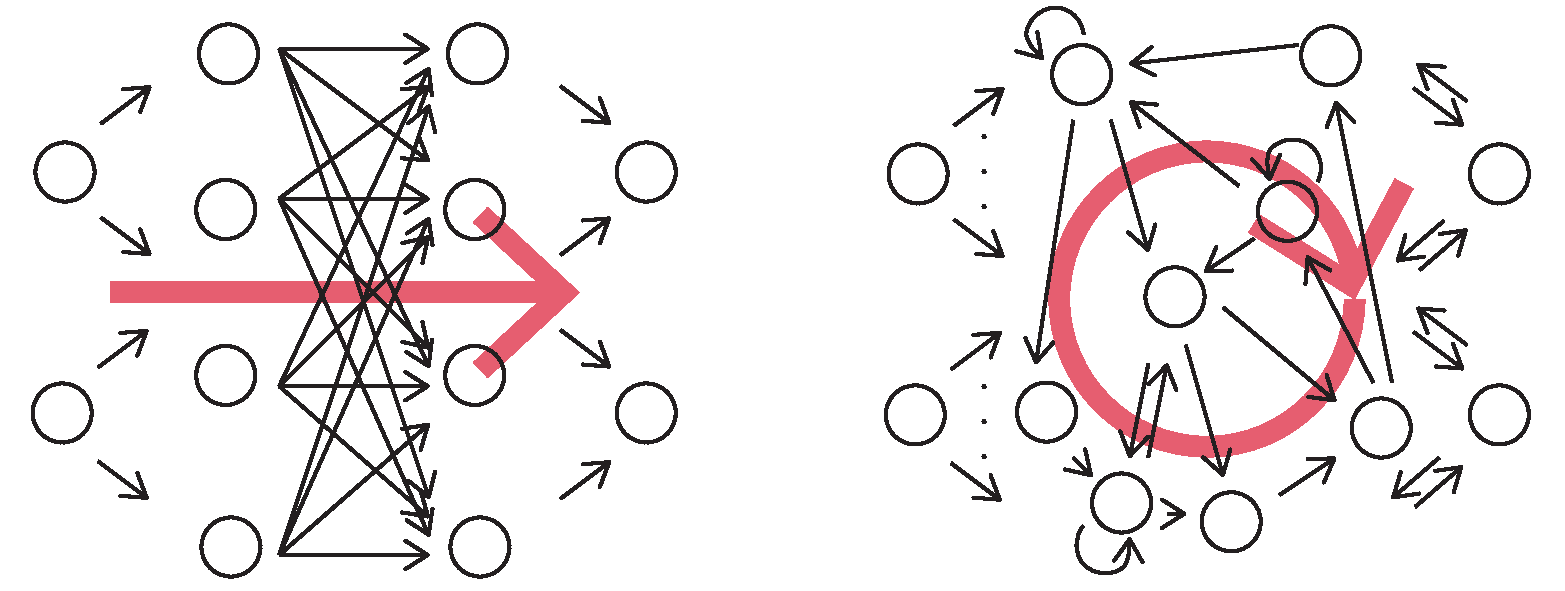
\includegraphics[width = 0.9 \textwidth]{figures/illustrations/ffnn_rnn_structure.pdf}
    \caption{Schematische Darstellung eines \textsc{FFNN} mit vier Ebenen (links) und eines \textsc{RNN} (rechts) mit ihren jeweiligen Verbindungen und der Eingangs- und Ausgangsebene. Der Informationsfluss ist in rot eingetragen (nach \citep{jeagerTut2002}).}
    \label{fig:ffnn_rnn_structure}
\end{figure}

Ein \textsc{RNN} hat einen ähnlichen Aufbau, doch hier können alle Einheiten an alle anderen Einheiten Signale weitergeben und von diesen erhalten. Die schematische Struktur ist im rechten Teil der Abbildung \ref{fig:ffnn_rnn_structure} dargestellt. Hierdurch erhält das Netzwerk eine Art Gedächtnisfunktion, wodurch temporale Strukturen verarbeitet und berücksichtigt werden können. Dies kann die Vorhersage in bestimmten Anwendungsbeispielen wie der Text- und Sprachanalyse verbessern.\\
Ein Nachteil ist, dass zum Trainieren, aufgrund der rekurrenten Struktur, nicht mehr der einfachere \textsc{Backpropagation}-Algorithmus genutzt werden kann, sondern eine für \textsc{RNN}s abgewandelte Form genutzt werden muss. Für den prominenteste Algorithmus werden die verschiedenen Zustände die das \textsc{RNN} im Laufe der Signal-Propagation annimmt nacheinander betrachtet und auf diese zeitliche Entwicklung anschließend der \textsc{Backpropagation}-Algorithmus angewendet. Diese Methode ist unter dem Namen \textsc{Backpropagation through Time} (BTT) bekannt. Sie ist zum einen rechenaufwendiger und zum anderen auch instabiler, da das Verschwindenden und auch das Explodieren des Gradienten der Kostenfunktion deutlich wahrscheinlicher als bei der gewöhnlichen \textsc{Backpropagation} ist \citep{pascanu, jeagerTut2002}. Da bei diesem Ansatz die Gewichte ebenfalls anhand des Gradienten der Kostenfunktion angepasst werden, wird der Algorithmus instabil, falls diese explodieren oder ineffizient, wenn sie verschwinden.

\section{Echo State Network}
\label{sc:esn}
\subsection{Überblick}
Um die (Leistungs)Probleme der \textsc{RNN} zu umgehen, wurden als mögliche Lösung die \textsc{Echo State Networks} von H. Jäger vorgeschlagen \cite{jaeger2010}. Etwa zeitgleich wurde von W. Maas das Modell der \textit{Liquid State Machines} vorgeschlagen. In diesem Modell steht der biologische Hintergrund im Fokus, doch sind die Ergebnisse denen der \textsc{Echo State Networks} sehr ähnlich \citep{Maass2011}. 

\subsection{Aufbau}
\label{sec:esn_structure}
Ein \textsc{ESN} ist eine Spezialform eines \textsc{RNN}s. Hierbei wird eine auf dem ersten Blick eigenartige Entscheidung getroffen: Während des gesamten Trainingsvorganges werden die Verbindungen der einzelnen Einheiten größtenteils nicht verändert. Es wird versucht durch das \textit{Echo} der vorherigen Signale, welche noch im Netzwerk gespeichert sind, diese Signale zu rekonstruieren - hieraus ergibt sich auch der Name \cite{lukoseviciusa2009}. Im Folgenden wird der Aufbau und anschließend die Funktionsweise eines solchen Netzwerkes nach \citep{jaeger2007} beschrieben.\\

Allgemein bildet das Netzwerk $S$ ein zeitliches Signal $\vec{u}(n) \in \mathbb{R}^{N_u}$  auf eine zeitlich variable Ausgabe $\vec{y}(n) \in \mathbb{R}^{N_y}$ für die Zeiten $n=1, ..., T$ ab. Zudem besitzt das System ein sogenanntes \textsc{Reservoir} aus $N$ nicht-linearen Einheiten. Der innere Zustand des Netzwerkes wird durch diese Einheiten beschrieben und als $s(n) \in \mathbb{R}^{N}$ bezeichnet.\\
Die Verbindungen der inneren Einheiten untereinander werden durch die Gewichtsmatrix $\mathbf{W} \in \mathbb{R}^{N \times N}$ beschrieben. Das Eingangssignal wird zusammen mit einem \textit{Bias} $b_{in} \in \mathbb{R}$ durch die Matrix $\mathbf{W_{in}} \in \mathbb{R}^{N \times (N_u+1)}$ auf die inneren Einheiten weitergeleitet.\\

Die zeitliche Entwicklung der inneren Zustände berechnet sich nach der Vorschrift
\begin{align}
\label{eq:esn_stateeq}
\vec{s}(n) = (1 - \alpha) \cdot \vec{x}(n-1)  + \alpha \cdot f_{in}\left( \mathbf{W_{in}} [b_{in}; \vec{u}(n)] + \mathbf{W} \vec{x}(n-1) \right),
\end{align}
wobei $f_{in}$ eine beliebige (meistens \textit{sigmoid}-förmige) Transferfunktion ist, und $[\cdot\,;\,\cdot]$ das vertikale Aneinanderfügen von Vektoren beziehungsweise Matrizen bezeichnet. Für diese Zustandsgleichung wurde das Modell eines \textit{Leaky Integrator Neurons} genutzt, wobei $\alpha \in (0,1]$ die Verlustrate beschreibt. Für $\alpha=1$ ergibt sich als Spezialfall ein gewöhnliches Neuron
\begin{align}
\vec{s}(n) = f_{in}\left( \mathbf{W_{in}} [b_{in}; \vec{u}(n)] + \mathbf{W} \vec{x}(n-1) \right).
\end{align}

Da für manche Anwendungsfälle auch eine direkte Rückkopplung wünschenswert ist, kann das System noch um eine Ausgabe-Rückkopplung erweitert werden. Diese verbindet die Ausgabe erneut mit den inneren Einheiten durch die Matrix $\mathbf{W_{fb}} \in \mathbb{R}^{N \times N_y}$.
Somit ergibt sich 
\begin{align}
\label{eq:esn_stateeq_feedback}
\vec{s}(n) = (1 - \alpha) \cdot \vec{x}(n-1)  \alpha \cdot f_{in}\left( \mathbf{W_{in}} [b_{in}; \vec{u}(n)] + \mathbf{W} \vec{x}(n-1) + \mathbf{W_{fb}} \vec{y}(n) \right)
\end{align}
als Zustandsgleichung. In Abbildung \ref{fig:esn_structure} ist der vollständige Struktur eines \textsc{ESN}s mit den Matrizen $\mathbf{W_{in}}, \mathbf{W}$ und $\mathbf{W_{out}}$ dargestellt.

\begin{figure}[H]
    \centering
    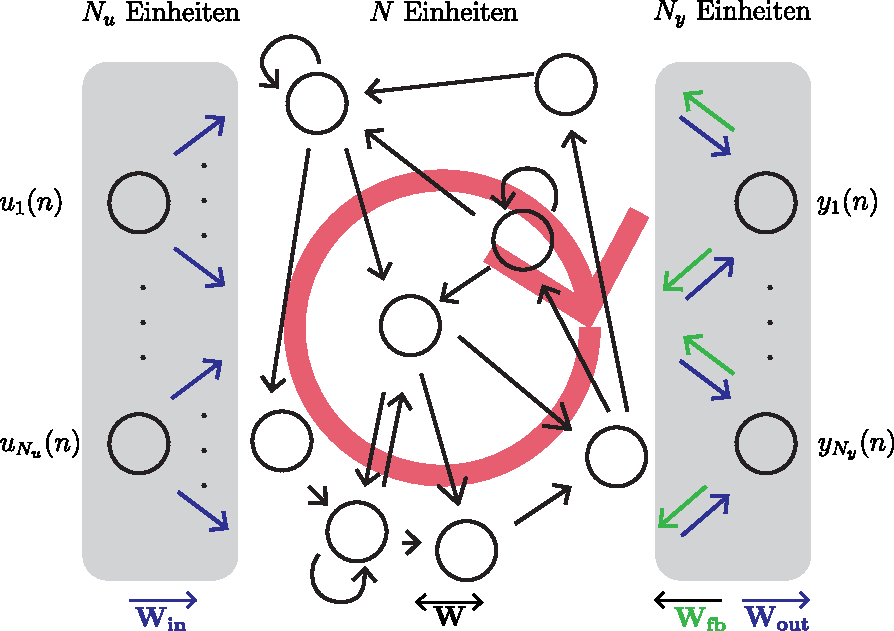
\includegraphics[width = 0.7 \textwidth]{figures/illustrations/esn_structure.pdf}
    \caption{Schematische Darstellung eines \textsc{ESN}. Von links nach rechts durchläuft das Eingangssignal $u(n)$ erst $N_u$ Eingangseinheiten, danach ein Reservoir mit $N$ Einheiten, bis schließlich die Ausgabe $y(n)$ mittels $N_y$ Ausgabeeinheiten gebildet wird. (nach \citep{jeagerTut2002, Ma2013}).}
    \label{fig:esn_structure}
\end{figure}


Anhand der inneren Zustände lassen sich nun noch die sogenannten erweiterten inneren Zustände $x(n) = [b_{out}; \vec{s}(n); \vec{u}(n)] \in \mathbb{R}^{1 + N_u + N}$ definieren, wobei $b_{out}$ ein \textit{Bias} für die Ausgabe darstellt. 

Aus diesen erweiterten inneren Zuständen kann nun die Ausgabe $\vec{y}(n)$ konstruiert werden. Dies kann entweder im Sinne einer Linearkombination durch die Ausgangsmatrix $\mathbf{W_{out}} \in \mathbb{R}^{(1 + N_u + N) \times N_y}$ oder durch andere nicht lineare Regressionsalgorithmen wie beispielsweise einer \textsc{Support Vector Machine (SVM)} durchgeführt werden. Im Folgenden wird nur der Fall einer Linearkombination betrachtet, da sich für die anderen Methoden ein analoges Verfahren ergibt.
In diesem Fall berechnet sich die Ausgabe mittels
\begin{align}
\vec{y}(n) = f_{out} \left( \mathbf{W_{out}} \vec{x}(n) = \mathbf{W_{out}} [b_{out}; \vec{s}(n); \vec{u}(n)] \right),
\end{align}
wobei $f_{out}$ die Transferfunktion der Ausgabe ist. Für diese kann in den meisten Fällen (so auch in dieser Arbeit) die Identität $f_{out}(x) = x$ genutzt werden.\\

Während die Matrix $\mathbf{W_{out}}$ durch den Trainingsvorgang bestimmt wird, werden die Matrizen $\mathbf{W_{in}}$ und $\mathbf{W}$ a priori generiert und festgelegt. Hierbei hat sich für das Generieren der Eingangsmatrix eine zufällige Anordnung von zufälligen Gleitkommazahlen zwischen $-0.5$ und $0.5$ als geschickt herausgestellt. Falls ein Feedback gewünscht ist, also Gleichung (\ref{eq:esn_stateeq_feedback}) genutzt wird, wird $\mathbf{W_{fb}}$ gleichartig konstruiert. Auf das Generieren der inneren Matrix $\mathbf{W}$ wird in Abschnitt \ref{sc:esn_theory} genauer eingegangen.

\subsection{Trainingsvorgang}
Nachdem der Aufbau des Netzwerkes beschrieben ist, ergibt sich nun die Frage, wie der Trainingsvorgang durchgeführt wird.

Hierfür wird für die Zeiten $n=0, ..., T_0$ das \textsc{ESN} mit dem Signal $\vec{u}(n)$ betrieben, wobei $T_0$ die \textit{transiente Zeit} beschreibt. Hierdurch soll das System aus seinem zufällig gewähltem Anfangszustand in einen charakteristischen Zustand übergehen. Anschließend wird das System für Zeiten $n < T$ weiter betrieben und die erweiterten Zustände $\vec{x}(n)$ als Spalten in der \textit{Zustandsmatrix} $\mathbf{X} \in \mathbb{R}^{(1 + N_u + N) \times T}$ gesammelt. Analog dazu werden die gewünschten Ausgaben $\vec{y}(n)$ nach dem Anwenden der Inversen $f^{-1}_{out}$ der Ausgabe-Transferfunktion $f_{out}$ auch als Spalten in der \textit{Ausgabematrix} $Y \in \mathbb{R}^{N_y \times T}$ gesammelt.
Nun wird eine Lösung der Gleichung
\begin{align}
\mathbf{Y} = \mathbf{W}_{out} \mathbf{X}
\end{align}
für $\mathbf{W}_{out}$ gesucht. Hierfür stehen mehrere Verfahren zur Verfügung, von denen zwei prominente erwähnt sein sollen.
Zum einen kann die Lösung durch eine \textit{Tikhonov Regularisierung} mittels der Regularisierung $\beta \cdot ||\vec{W}_{out, i}||^2$ der Gewichtsmatrix mit der Konstante $\beta$ erhalten werden. Hierbei steht $\vec{W}_{out, i}$ für die jeweils $i$-te Zeile der Gewichtsmatrix. Das Verfahren
\begin{align}
\label{eq:tikhonov}
\mathbf{W}_{out} = \mathbf{Y} \mathbf{X}^T \left(\mathbf{X} \mathbf{X}^T + \beta I \right)^{-1}
\end{align}
ist sehr leistungsstark, aber auch teilweise numerisch instabil. Bei geeigneter Wahl von $\beta$ können die besten Ergebnisse hinsichtlich der Genauigkeit der Vorsage erzielt werden \cite{lukoseviciusa2009}. Deshalb wird in dieser Arbeit auch nur dieses Lösungsverfahren verwendet. Die weiteren Lösungsansätze für das Gleichungssystem sind nur aus Gründen der Vollständigkeit angegeben.\\

Zum anderen kann zur Lösung die \textit{Moore-Penrose-Pseudoinverse} $\mathbf{X}'$ genutzt werden, sodass für die Ausgabematrix
\begin{align}
\label{eq:pseudo_inverse}
\mathbf{W}_{out} = \mathbf{Y} \mathbf{X}'
\end{align}
folgt. Dieses Verfahren ist zwar sehr rechenaufwendig aber dafür numerisch stabil \cite{lukoseviciusa2009, jaeger2012}. Nichts desto trotz, kann allerdings auf Grund des Fehlens einer Regularisierung leicht der Effekt des \textsc{Overfittings} auftreten. Auf Grund dessen wird es in dieser Arbeit nicht verwendet.\\

Um den Effekt des Overfittings bei der Verwendung der Psuedoinversen zu reduzieren, kann in der Zustandsgleichung (\ref{eq:esn_stateeq}) beziehungsweise (\ref{eq:esn_stateeq_feedback}) eine leichte normalverteilte Störung $\vec{\nu}(n)$ der Größenordnung $\num{1e-1}$ bis $\num{1e-5}$ addiert wird. Falls die \textit{Tikhonov Regularisierung} zur Lösung verwendet wird, erhöht die Verwendung der zufälligen Störung die Stabilität der Vorhersage des System. Dieser Ansatz beruht auf Empirie, da eine mathematische Begründung hierfür noch nicht vollständig gelungen ist \citep{jaeger2010, lukoseviciusa2009}. Anschaulich lässt sich das Vorgehen dadurch motivieren, dass hierdurch künstliche Datenpunkte in der nähe der vorhandenen Trainingsdaten emuliert werden, und somit eine größere Vielfalt an Daten während der Trainingsphase beobachtet wird.\\

Zusammenfassend ergibt sich somit der folgende Funktionsablauf für die Anwendung eines \textsc{ESN}:

\singlespacing
\begin{enumerate}
	\item Zufälliges Generieren der Matrizen $\mathbf{W}_{in}, \mathbf{W}_{fb}$ und Konstruktion der Matrix $\mathbf{W}$ 
	\item Einspeisen des Signals $u(n)$ und Konstruktion der Zustandsmatrix $\mathbf{X}$ und der Ausgabematrix $\mathbf{Y}$ 
	\item Berechnung der Ausgabematrix $\mathbf{W}_{out}$
	\item Einspeisen des Signals $u(n)$ für Vorhersagen des Signales $y(n)$ für $n > T$
\end{enumerate}
\onehalfspacing

Zusätzlich zu diesen Eigenschaften wird die Dynamik des Reservoirs auch von dessen Größe $N$ bestimmt. Es kann gezeigt werden, dass die Gedächtnisleistung eines Reservoirs stark von dieser abhängt. Somit ist es ratsam für Aufgaben, die eine lange Gedächtnisleistung benötigen, ein großes und für Aufgaben, die nur ein Kurzzeitgedächtnis benötigten, ein kleines Reservoir zu benutzen \citep{jeagerTut2002}.





\subsection{Theoretischer Hintergrund}
\label{sc:esn_theory}
Um die mathematischen Eigenschaften beschreiben zu können, sind zuerst zwei Definitionen nötig \cite{yildiz}.

\begin{definition}[Kompatibler Zustand]
Sei $S : X \times U \rightarrow X$ ein \textsc{ESN} mit der Zustandsgleichung $\vec{x}_{n+1} = F \left( \vec{x}_n, \vec{u}_{n+1} \right)$. Eine Folge von Zuständen $(\vec{x}_n)_n$ ist kompatibel mit der Eingangsfolge $(\vec{u}_n)_n$, wenn $\vec{x}_{n+1} = F\left( \vec{x}_n, \vec{u}_{n+1} \right), \forall n \leq 0$ erfüllt ist.
\end{definition}

\begin{definition}[Echo State Eigenschaft (ESP)]
Ein \textsc{ESN} $S : X \times U \rightarrow X$ besitzt die \textit{Echo State Eigenschaft} genau dann wenn eine Nullfolge $(\delta_n)_{n \geq 0}$ existiert, sodass für alle Zustandsfolgen $(\vec{x}_n)_n, (\vec{x}'_n)_n$ die kompatibel mit der Eingangsfolge $(\vec{u}_n)_n$ sind gilt, dass $\forall n \geq 0 ||x_n - x'_n|| < \delta_n$
\end{definition} 
Dies bedeutet, dass nachdem das Netzwerk lang genug betrieben worden ist, der Zustand nicht mehr von dem beliebig gewähltem Anfangszustand abhängt. Diese Eigenschaft ist notwendig, damit das \textsc{ESN} Vorhersagen treffen kann \cite{jeagerTut2002}.\\

Nun stellt sich die Frage, wann ein Netzwerk diese Eigenschaft besitzt. Es wird schnell klar, dass dies hauptsächlich durch die Gewichtsmatrix $\mathbf{W}$ bestimmt wird. Betrachtet man die Zustandsgleichung des Netzwerkes, so lässt sich auf Grund des \textit{Banachschen Fixpunktsatzes} erkennen, dass die \textit{ESP} für alle Eingänge $\vec{u}_n$ vorliegt, sobald $||\vec{x}_{n+1} - \vec{x}'_{n+1}|| < ||\vec{x}_n - \vec{x}'_n||$ für zwei kompatible Zustände $\vec{x}_n \neq \vec{x}'_n$ erfüllt ist \cite{jaeger2010}.
Hieraus ergibt sich, dass die \textit{ESP} vorliegt, wenn 
\begin{align}
\label{eq:theory_old_requirement}
|1-\alpha(1-\sigma_{max}(\mathbf{W}))| < 1
\end{align}
erfüllt ist, wobei $\sigma_{max}(\mathbf{W})$ der größte Singulärwert ist \cite{jaeger2007}.\\
Weitergehend ist bekannt, dass für Systeme bei denen der Spektralradius $\rho(\mathbf{W}) > 1$ ist diese Eigenschaft nicht vorliegen kann, sofern $\vec{u}_n = 0$ möglich ist \cite{jaeger2007, jaeger2010}.\\

Hieraus ergab sich lange Zeit die falsche Annahme, dass für Systeme mit $\rho(\mathbf{W}) < 1$ die Eigenschaft stets garantiert ist. Wie allerdings gezeigt werden konnte, ist dies nicht der Fall \citep{yildiz}. Stattdessen konnte gezeigt werden, dass eine hinreichende Bedingung durch
\begin{align}
\label{eq:theory_sufficient_requirement}
\rho(\alpha |\mathbf{W}|+(1-\alpha) \mathbf{I}) < 1
\end{align}
gegeben ist - wobei als Betrag der Matrix hier das elementweise Betragsnehmen gemeint ist. Diese Bedingung ist weniger einschränkend als Gleichung (\ref{eq:theory_old_requirement}) \cite{yildiz}.\\

Weitergehend hat sich in Experimenten gezeigt, dass eine dünnbesetze Gewichtsmatrix $\mathbf{W}$ zu reicheren Dynamiken innerhalb des Reservoirs führen kann \citep{jaeger2010}. Eine solche dünnbesetze Matrix bedeutet, dass nicht mehr jedes Neuron mit jedem anderen Neuron verbunden ist, sondern dass nur noch ein relativer Anteil $\epsilon$ dieser Verbindungen vorhanden ist. Da durch eine größere Anzahl an verschiedenen internen Dynamiken vielfältigere Funktionen besser approximiert werden können, kann die Vorhersagequalität durch einen Geringen $\epsilon$ Wert erhöht werden.\\

Darauf basierend kann nun eine Methode nach \cite{yildiz} angegeben werden, um die Gewichtsmatrix $\mathbf{W}$ zu konstruieren:

\singlespacing
\begin{enumerate}
	\item Generiere zufällige Matrix $\mathbf{W}$ mit $\mathbf{|W|} = \mathbf{W}$ bei der in jeder Zeile nur $\epsilon$ Einträge ungleich $0$ sind.
	\item Skaliere $\mathbf{W}$, sodass Gleichung (\ref{eq:theory_sufficient_requirement}) erfüllt ist.
	\item Wechsel zufällig das Vorzeichen von ungefähr der Hälfte aller Einträge.
\end{enumerate}
\onehalfspacing

Statt dieser Vorschrift wurde zuvor oftmals $\mathbf{W}$ zufällig generiert und anschließend nur $\rho(\mathbf{W})$ statt $\rho(|\mathbf{W}|)$ skaliert, was mit unter zu instabilen Systemen geführt hat. Da allerdings auch für Systeme mit einem Spektralradius $ > 1$ die \textit{ESP} beobachtet werden kann für nicht verschwindende Eingänge $\vec{u}_n$, ist es ratsam auch effektive Spektralradien jenseits $1$ auszuprobieren.